% ---- full-coverage figures (work2/code/table_figures_full.py) ----
% Every number printed in the source table is drawn here; verify_full() checks this.

\begin{figure*}[!tbp]
\centering
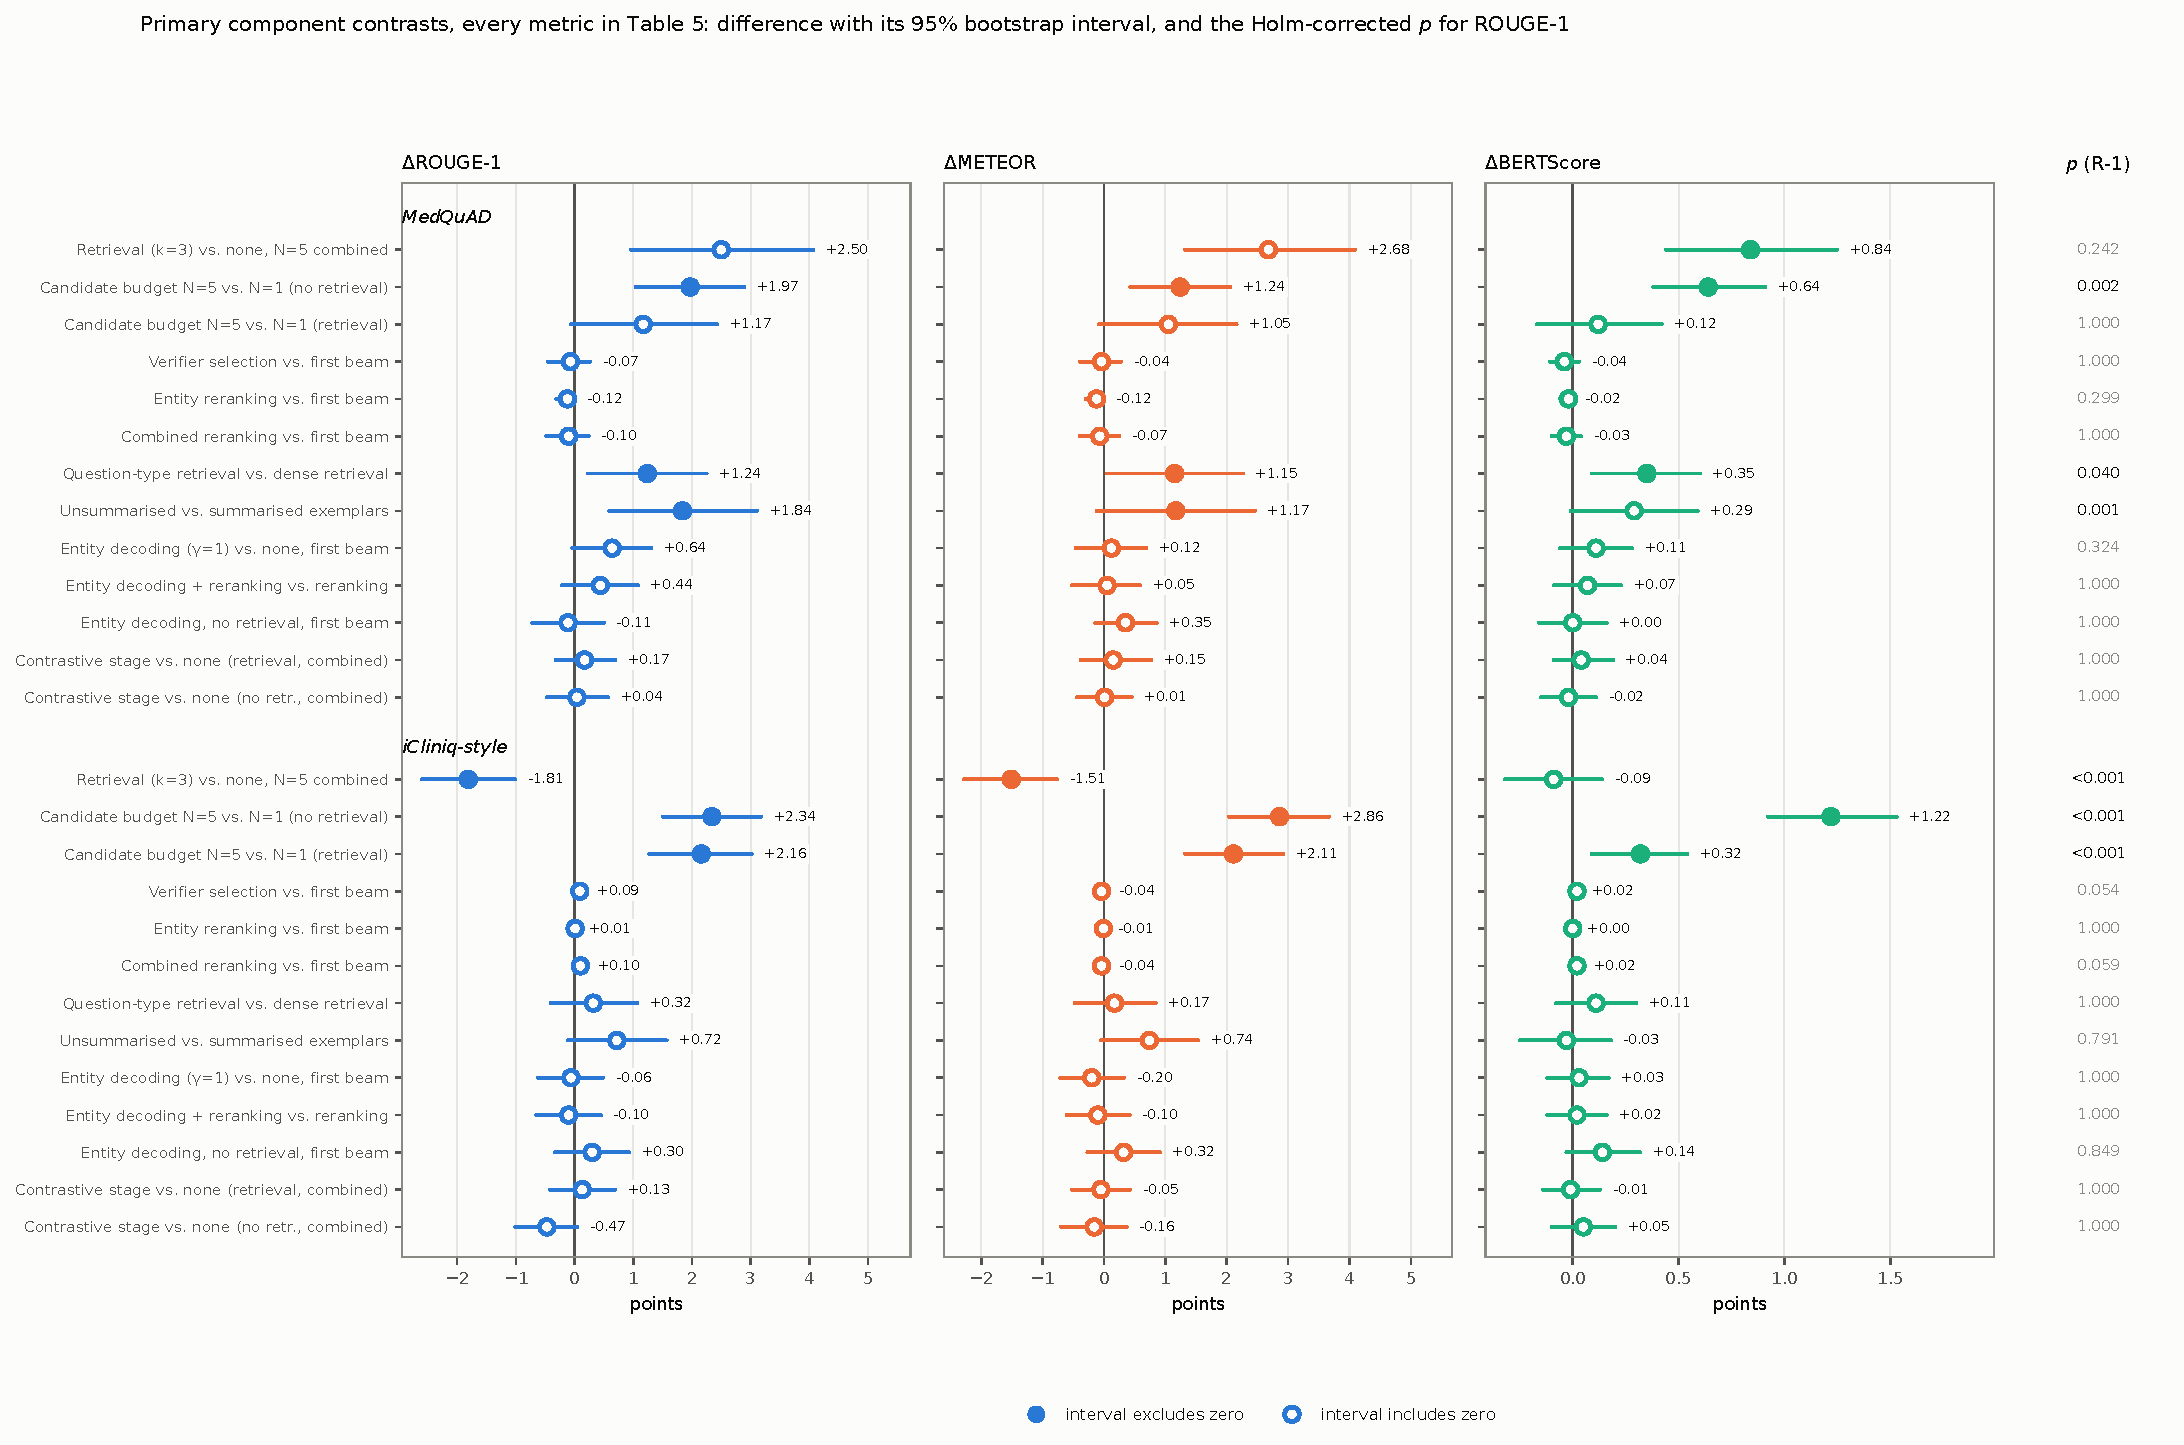
\includegraphics[width=\linewidth]{figures/tab5_primary_components_full.pdf}
\caption{Primary component contrasts, every column of Table~\ref{tab:primary-components}: $\Delta$ROUGE-1, $\Delta$METEOR and $\Delta$BERTScore, each with its 95\% bootstrap interval, and the Holm-corrected $p$. A filled marker means the interval excludes zero.}
\label{fig:tab5-primary-components-full}
\end{figure*}

\begin{figure*}[!tbp]
\centering
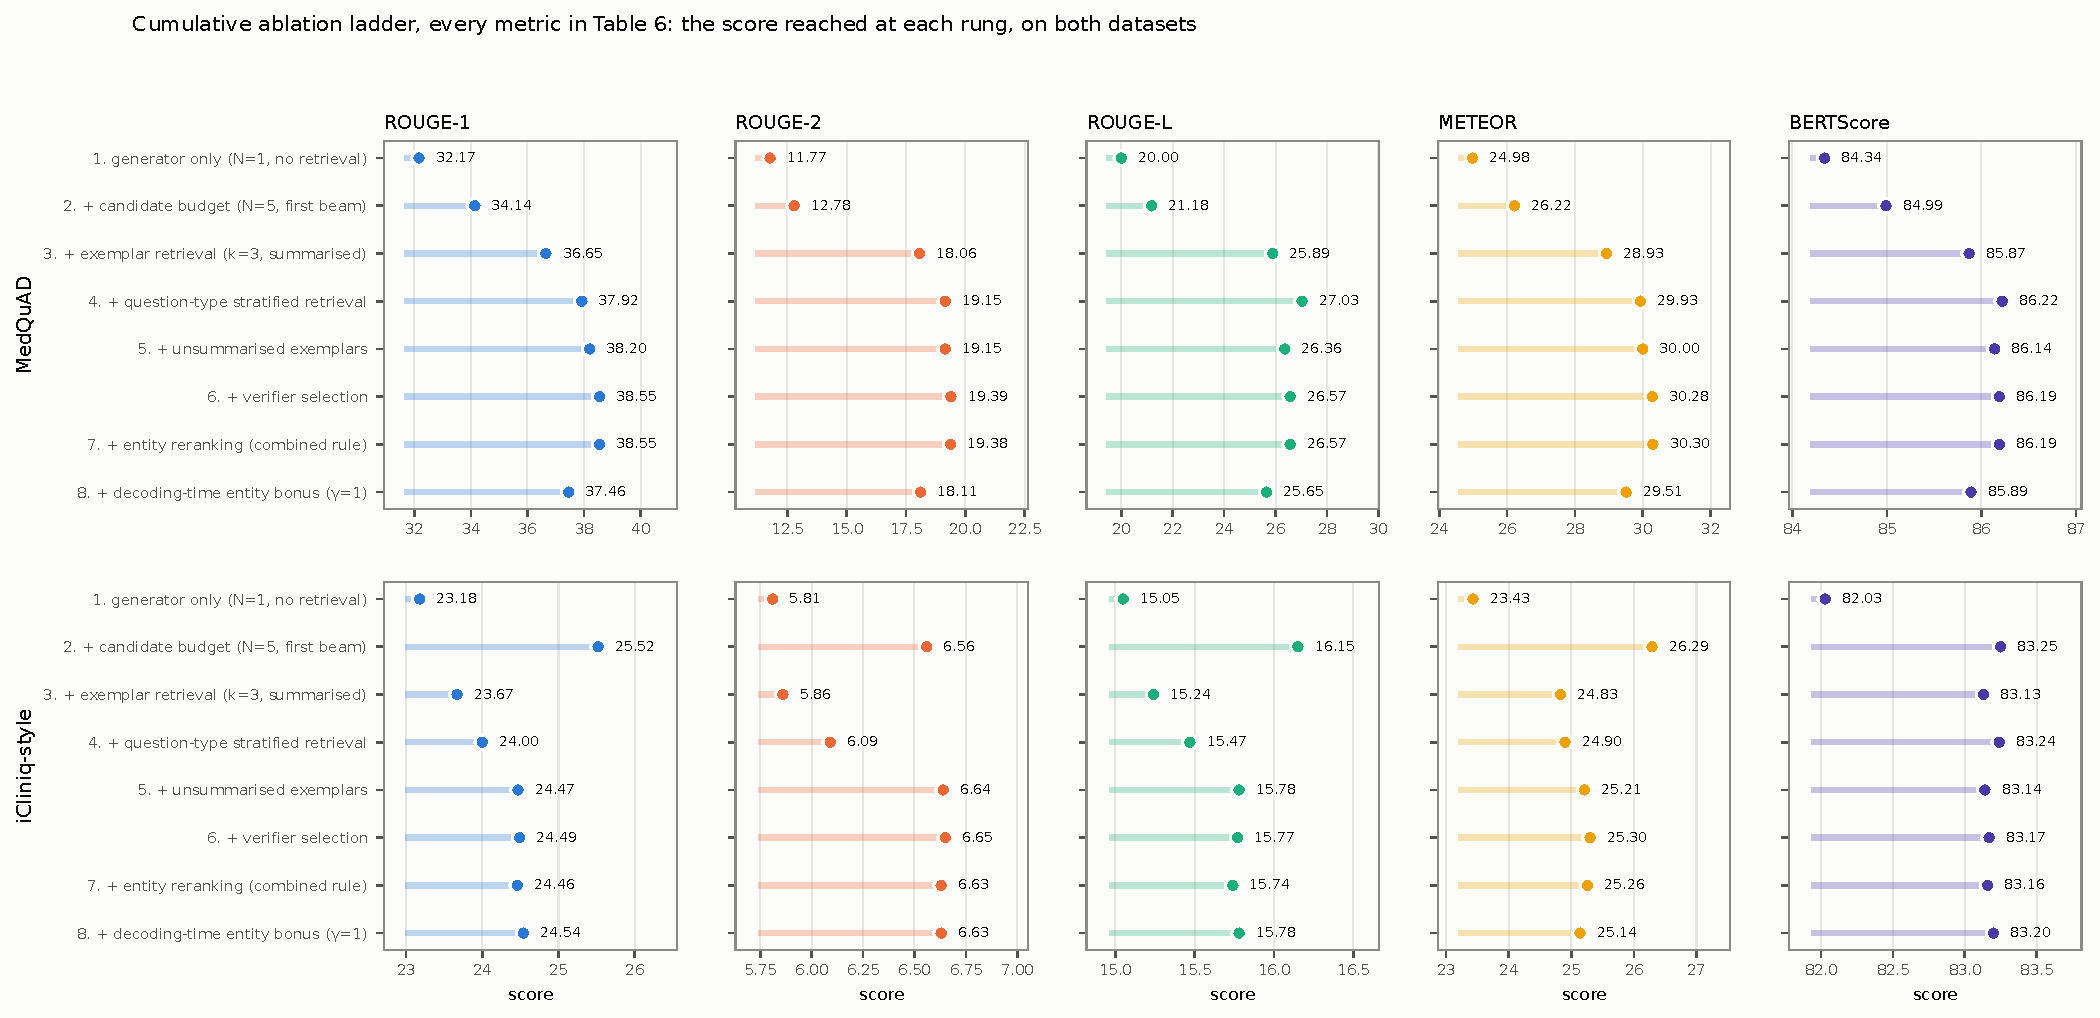
\includegraphics[width=\linewidth]{figures/tab6_ladder_levels_full.pdf}
\caption{Cumulative ablation ladder, every column of Table~\ref{tab:ladder-levels}: the level reached at each rung on all five metrics, on both datasets.}
\label{fig:tab6-ladder-levels-full}
\end{figure*}

\begin{figure*}[!tbp]
\centering
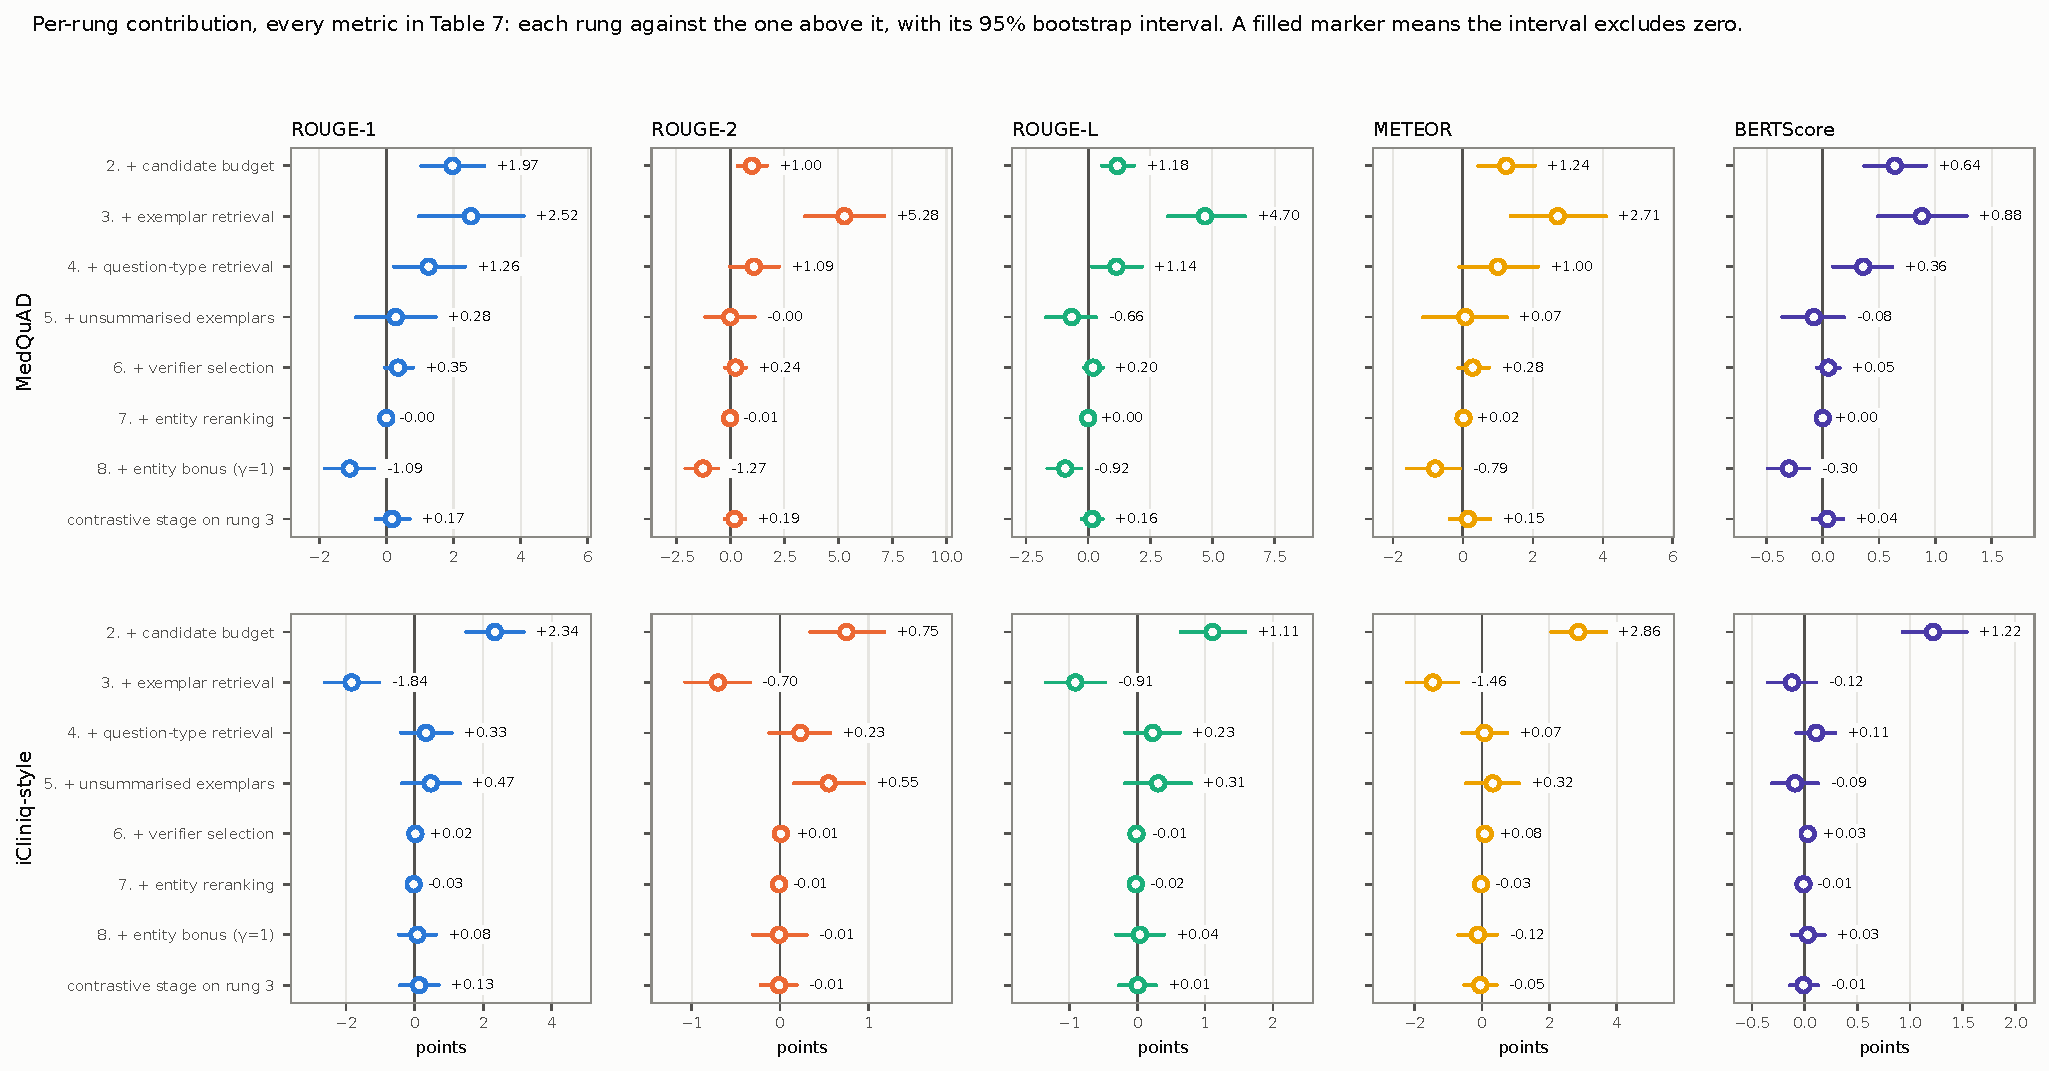
\includegraphics[width=\linewidth]{figures/tab7_ladder_steps_full.pdf}
\caption{Per-rung contribution, every column of Table~\ref{tab:ladder-steps}: each rung against the one above it on all five metrics, with 95\% bootstrap intervals.}
\label{fig:tab7-ladder-steps-full}
\end{figure*}

\begin{figure*}[!tbp]
\centering
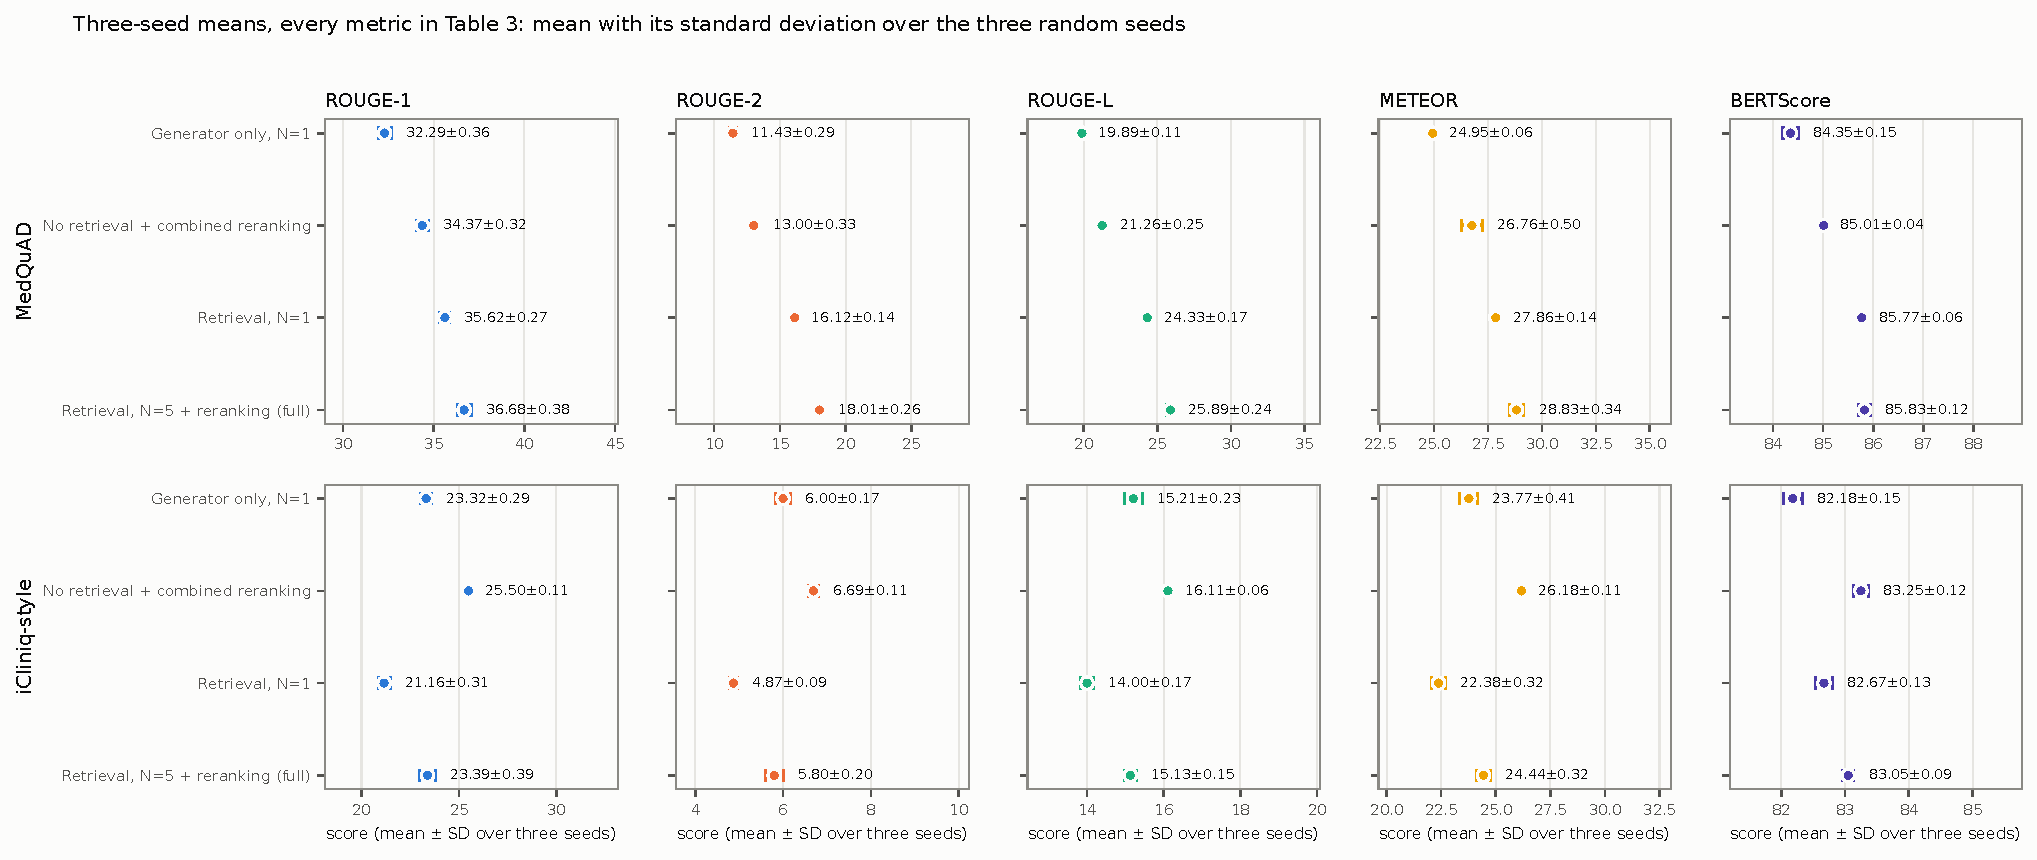
\includegraphics[width=\linewidth]{figures/tab3_seeds_full.pdf}
\caption{Three-seed means, every column of Table~\ref{tab:seeds}: mean and standard deviation over seeds for all five metrics.}
\label{fig:tab3-seeds-full}
\end{figure*}

\begin{figure*}[!tbp]
\centering
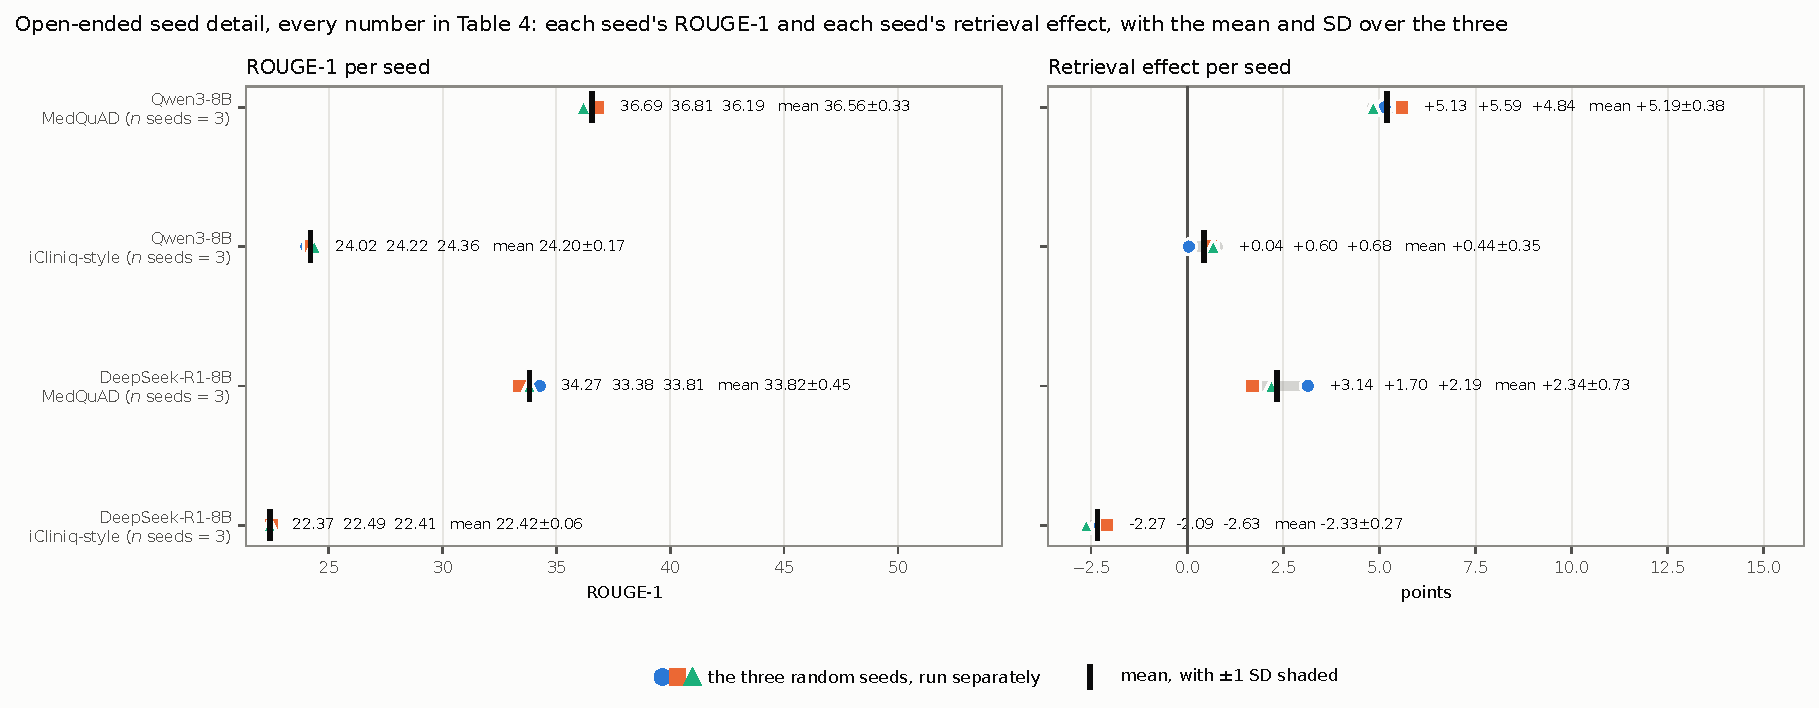
\includegraphics[width=\linewidth]{figures/tab4_open_seeds_full.pdf}
\caption{Open-ended seed detail, every column of Table~\ref{tab:open-seeds}: each seed's ROUGE-1 and each seed's retrieval effect, with mean and SD.}
\label{fig:tab4-open-seeds-full}
\end{figure*}

\begin{figure*}[!tbp]
\centering
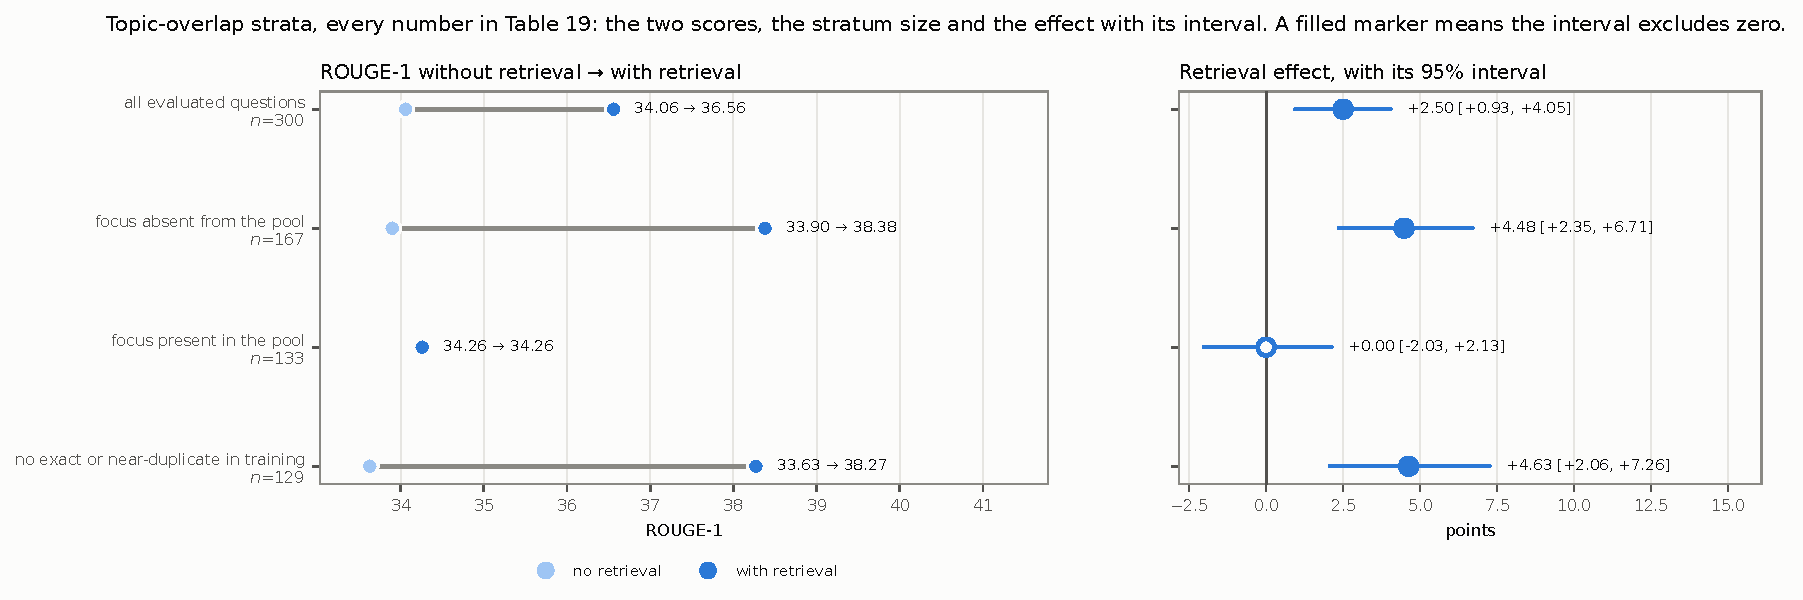
\includegraphics[width=\linewidth]{figures/tab19_topic_strata_full.pdf}
\caption{Topic-overlap strata, every column of Table~\ref{tab:topic}: stratum size, the two scores and the retrieval effect with its interval.}
\label{fig:tab19-topic-strata-full}
\end{figure*}

\begin{figure*}[!tbp]
\centering
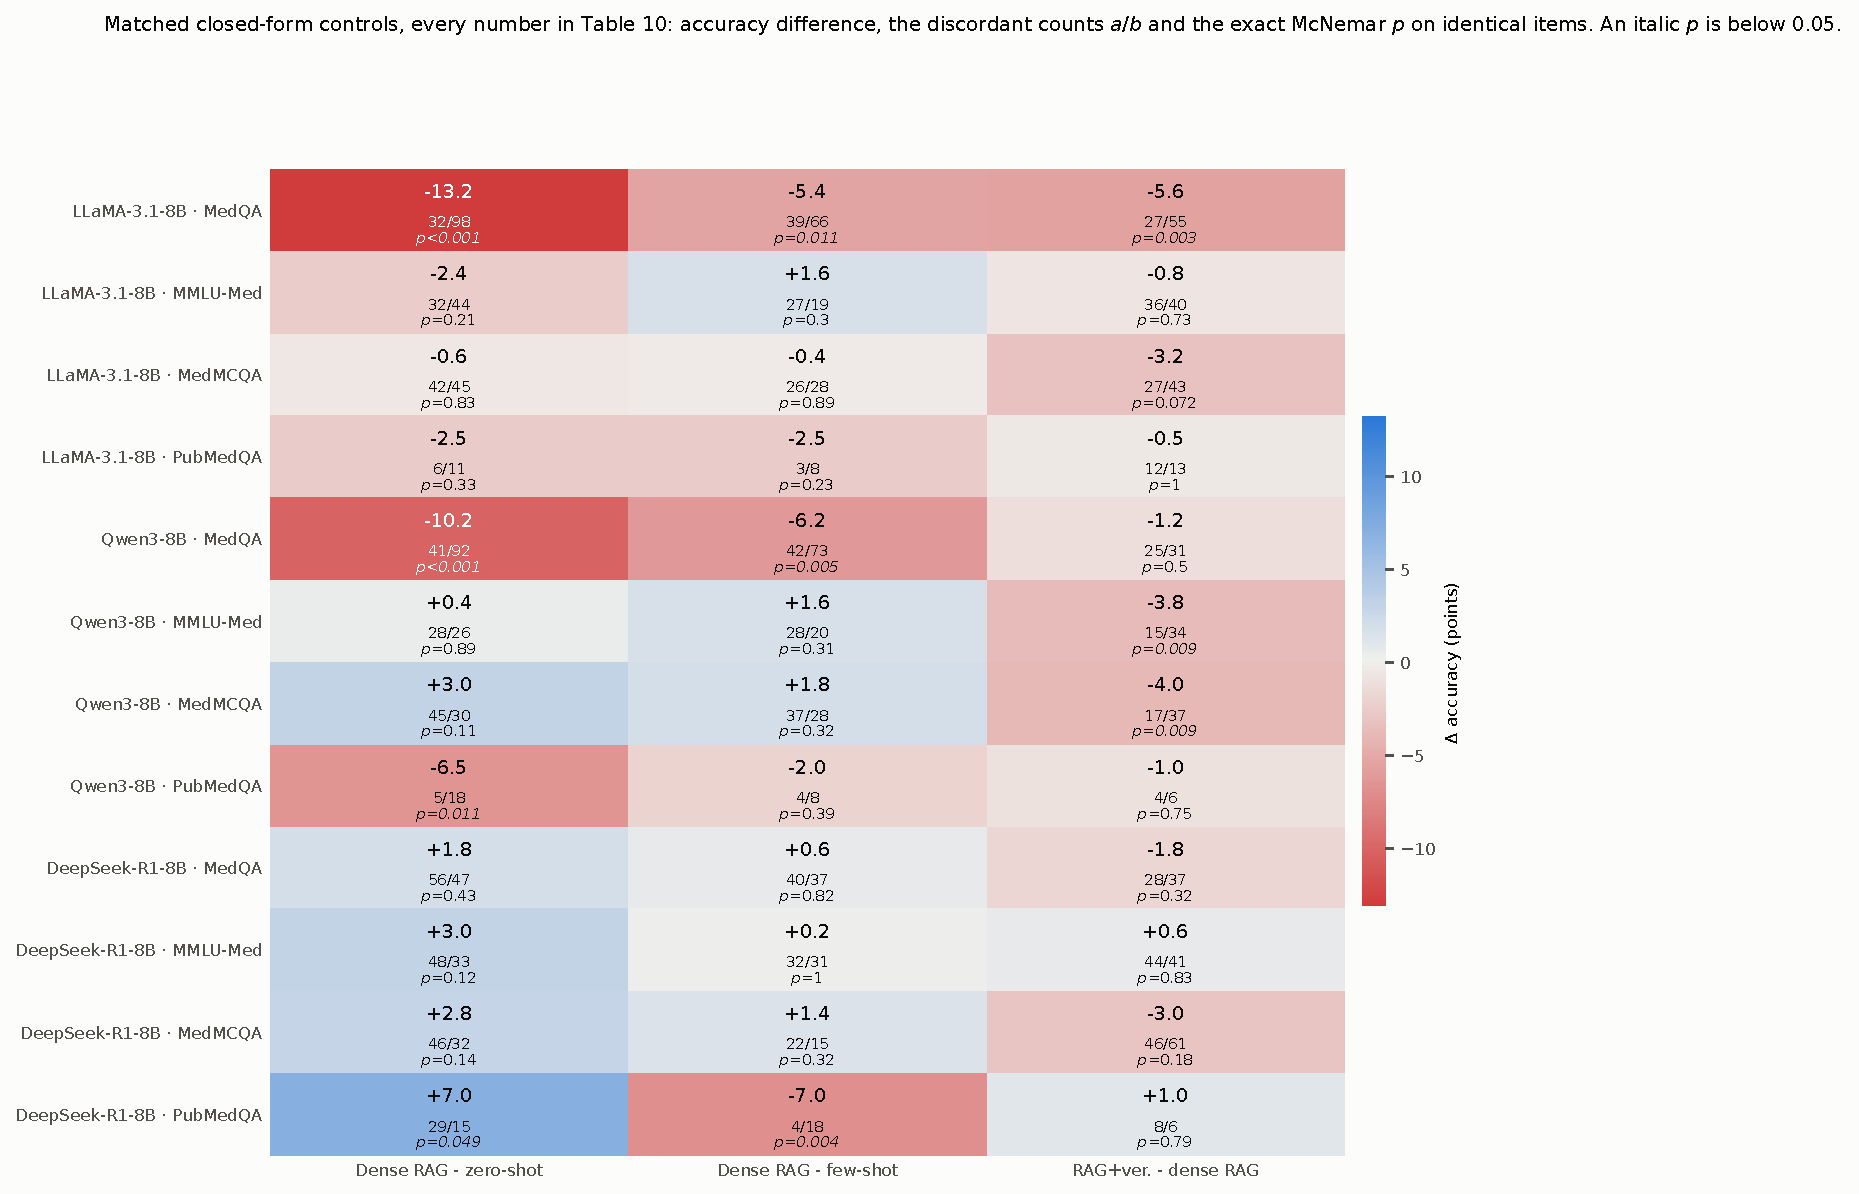
\includegraphics[width=\linewidth]{figures/tab10_closedform_matched_full.pdf}
\caption{Matched closed-form controls, every number of Table~\ref{tab:cf-matched-paired}: accuracy difference, discordant counts $a/b$ and exact McNemar $p$ on identical items.}
\label{fig:tab10-closedform-matched-full}
\end{figure*}

\begin{figure*}[!tbp]
\centering
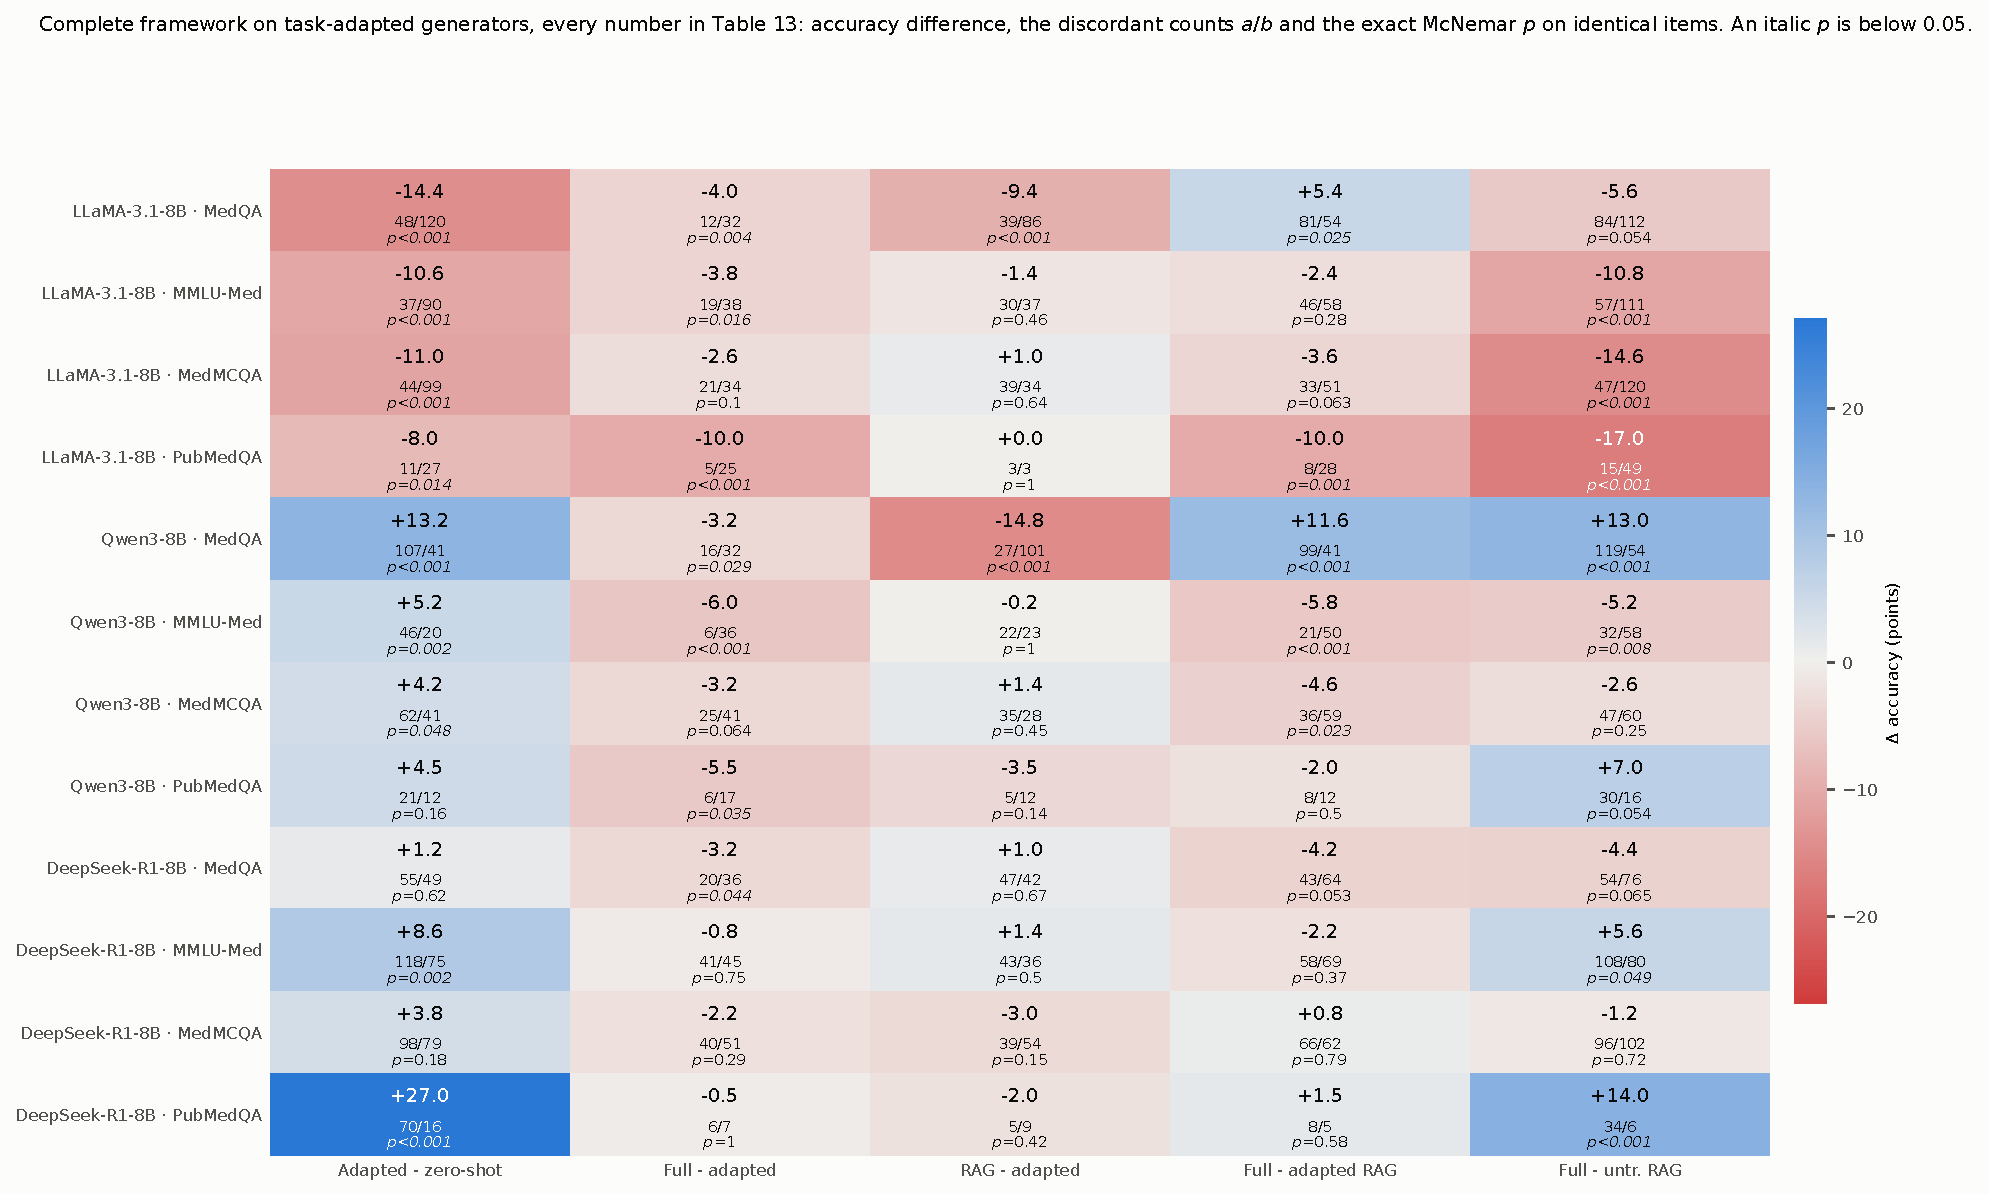
\includegraphics[width=\linewidth]{figures/tab13_closedform_full_full.pdf}
\caption{Complete framework on task-adapted generators, every number of Table~\ref{tab:cf-full-paired}: accuracy difference, discordant counts $a/b$ and exact McNemar $p$ on identical items.}
\label{fig:tab13-closedform-full-full}
\end{figure*}

\begin{figure*}[!tbp]
\centering
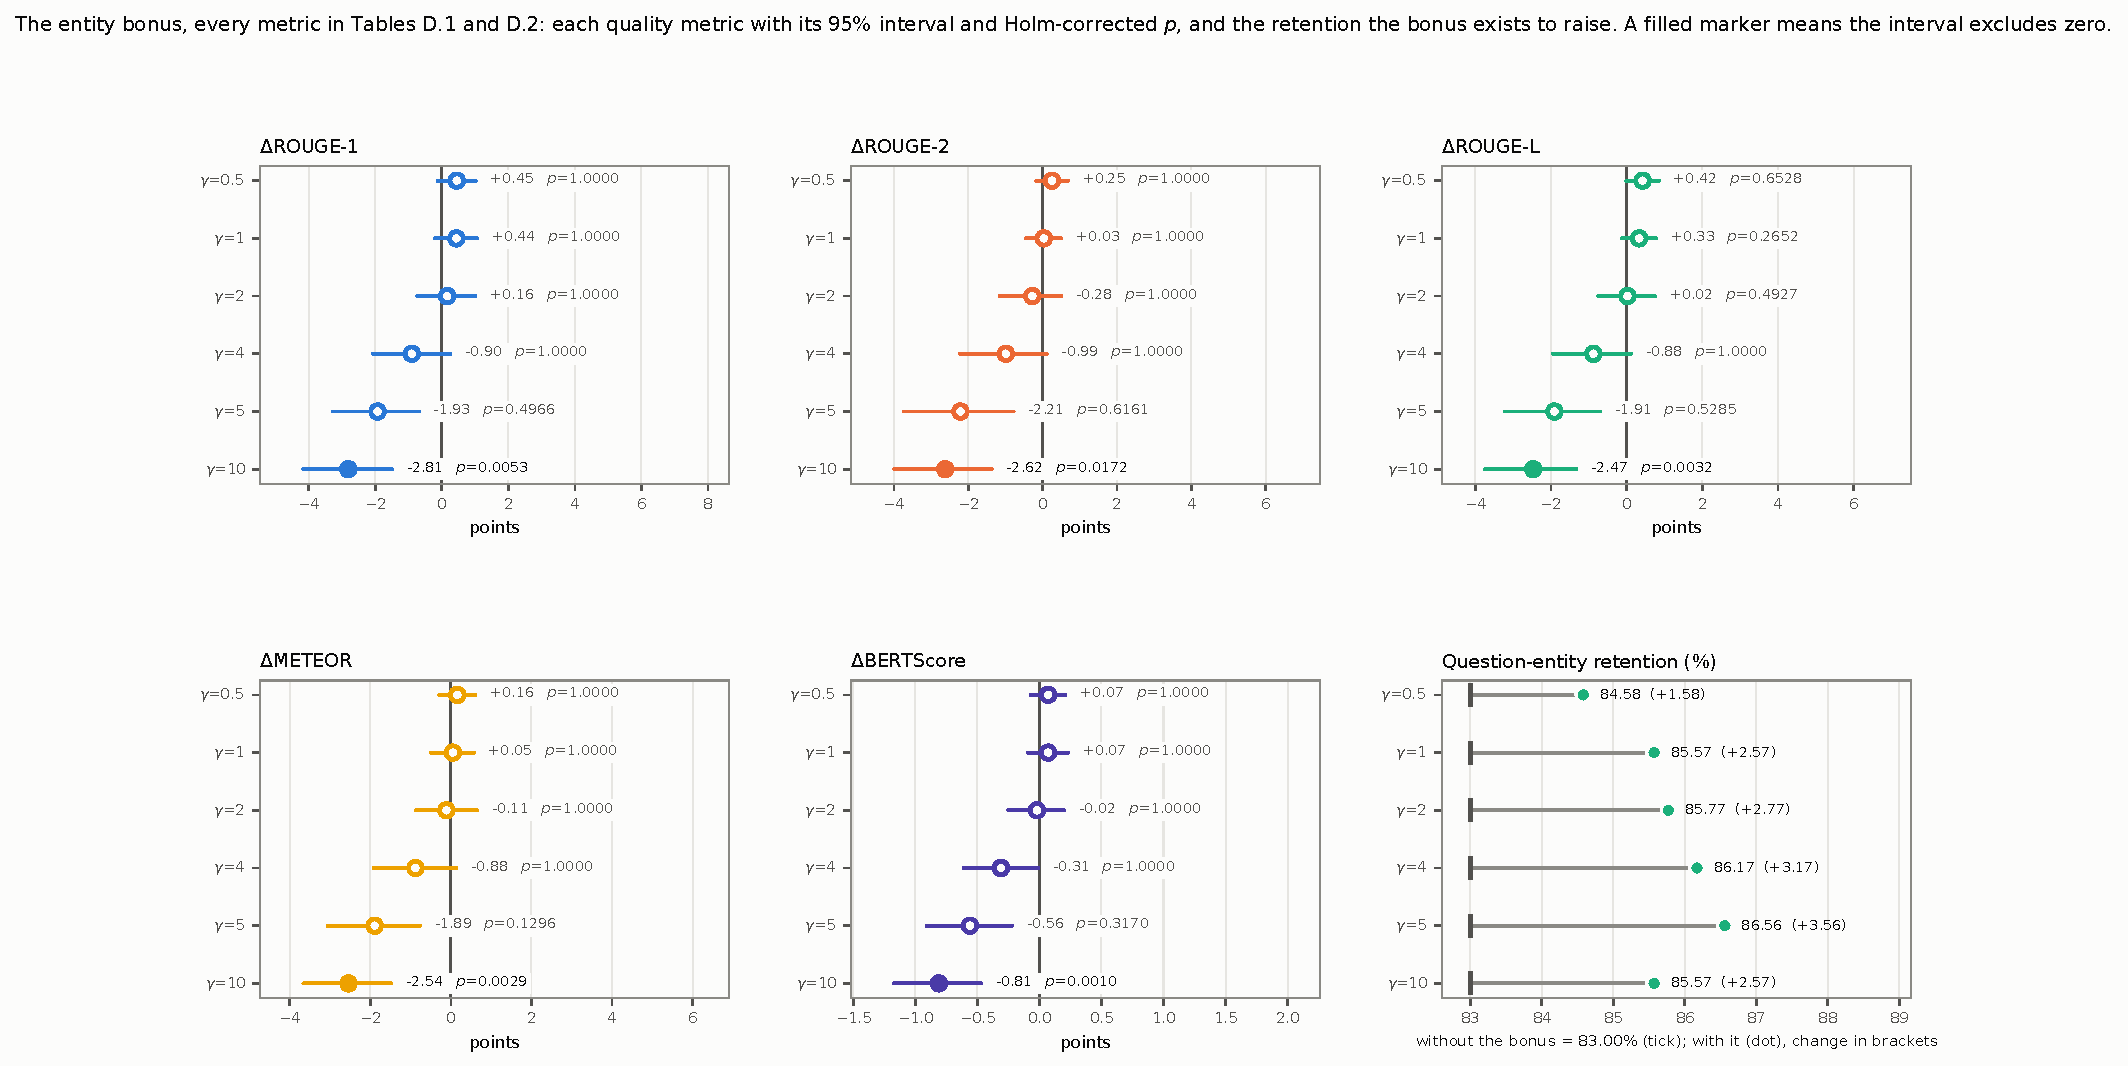
\includegraphics[width=\linewidth]{figures/tabD1_D2_gamma_sweep_full.pdf}
\caption{The entity bonus, every number of Tables~\ref{tab:gamma-sweep} and \ref{tab:gamma-retention}: five quality metrics with intervals and Holm-corrected $p$, and question-entity retention.}
\label{fig:tabD1-D2-gamma-sweep-full}
\end{figure*}

\begin{figure*}[!tbp]
\centering
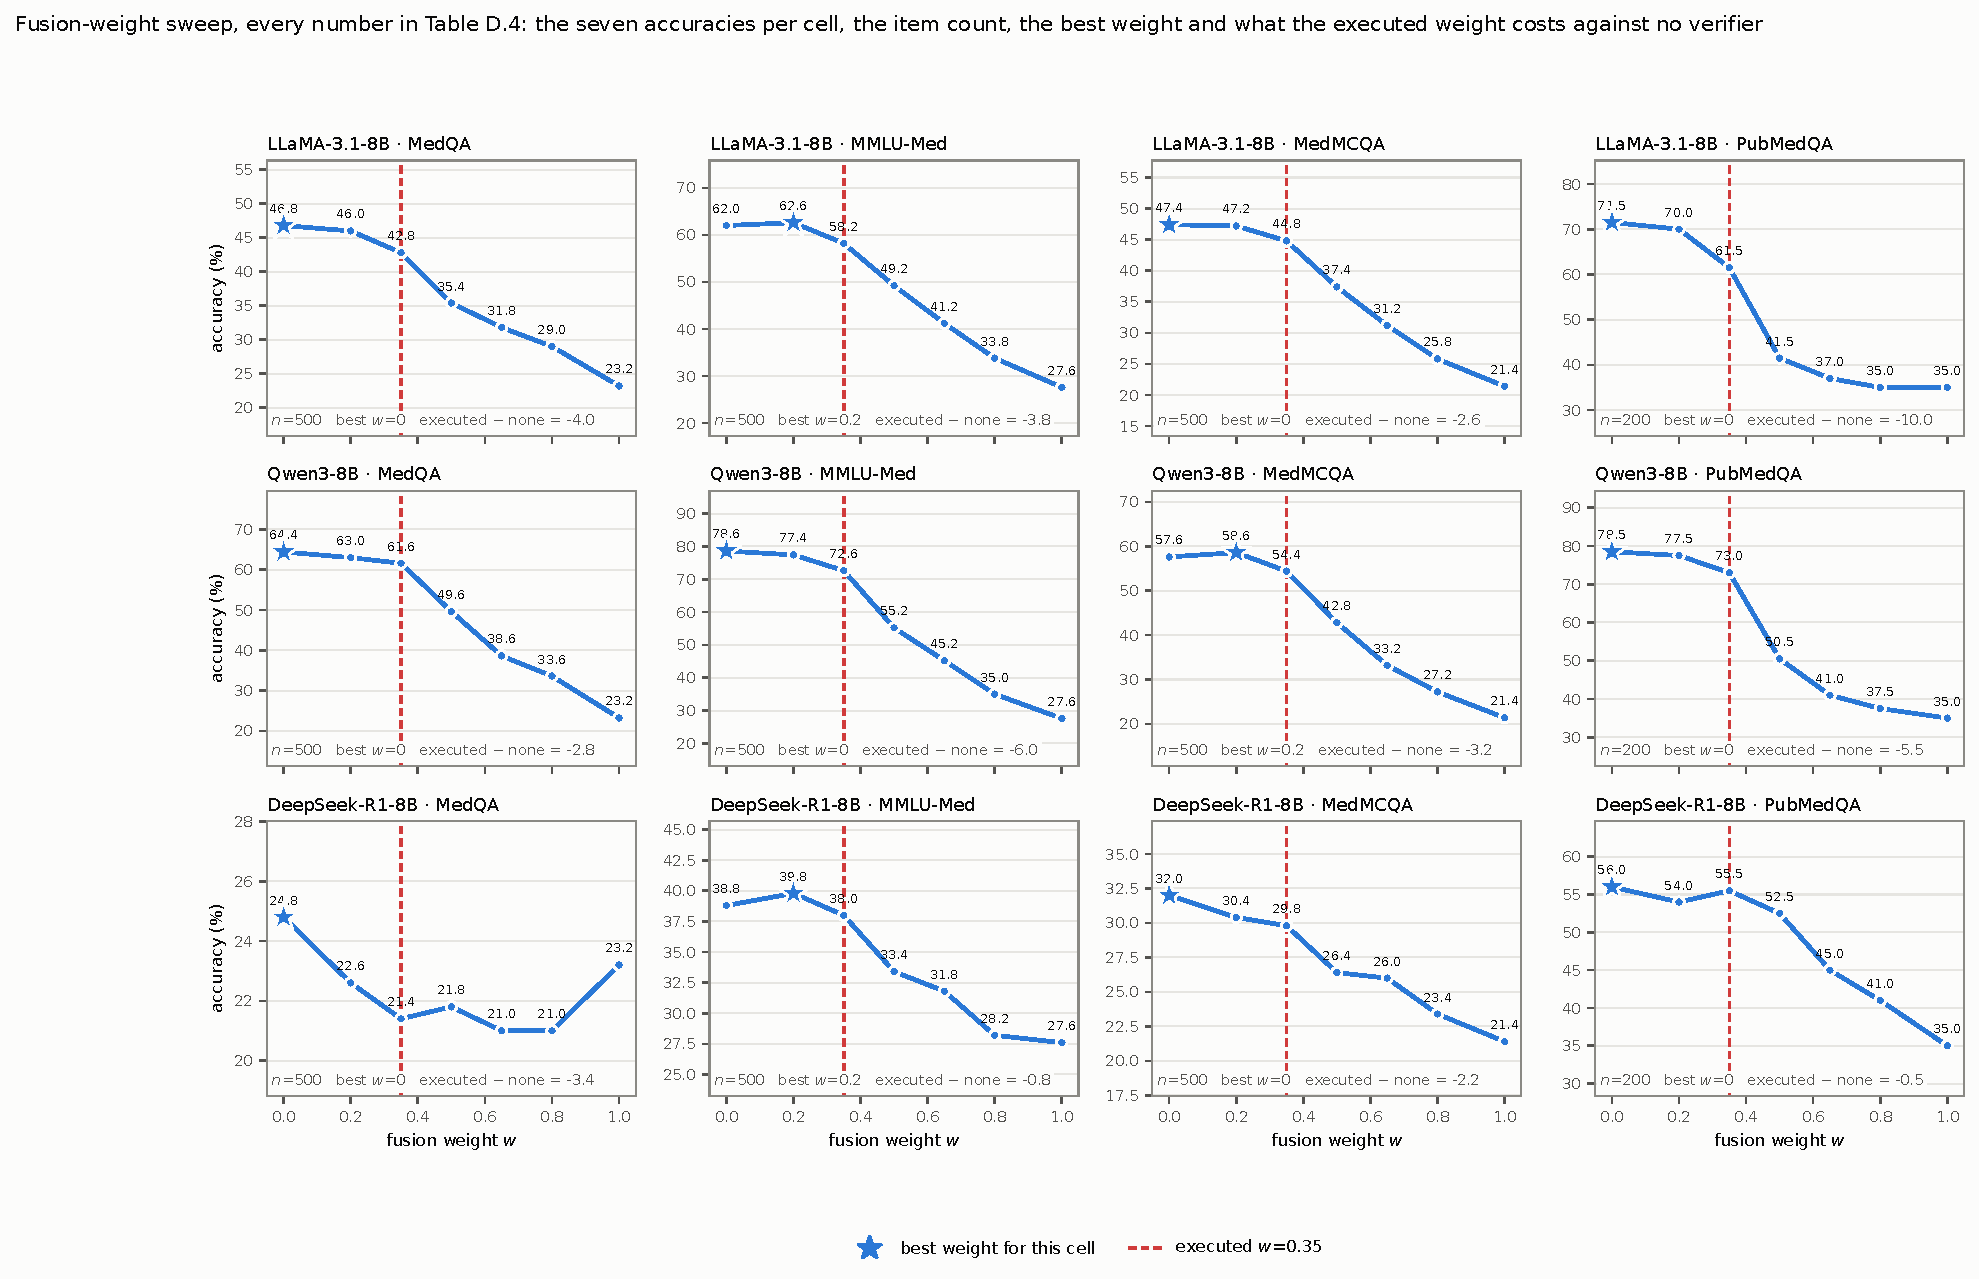
\includegraphics[width=\linewidth]{figures/tabD4_fusion_weight_sweep_full.pdf}
\caption{Fusion-weight sweep, every column of Table~\ref{tab:cf-weight-sweep}: the seven accuracies per cell, the item count, the best weight and the cost of the executed weight.}
\label{fig:tabD4-fusion-weight-sweep-full}
\end{figure*}

\begin{figure*}[!tbp]
\centering
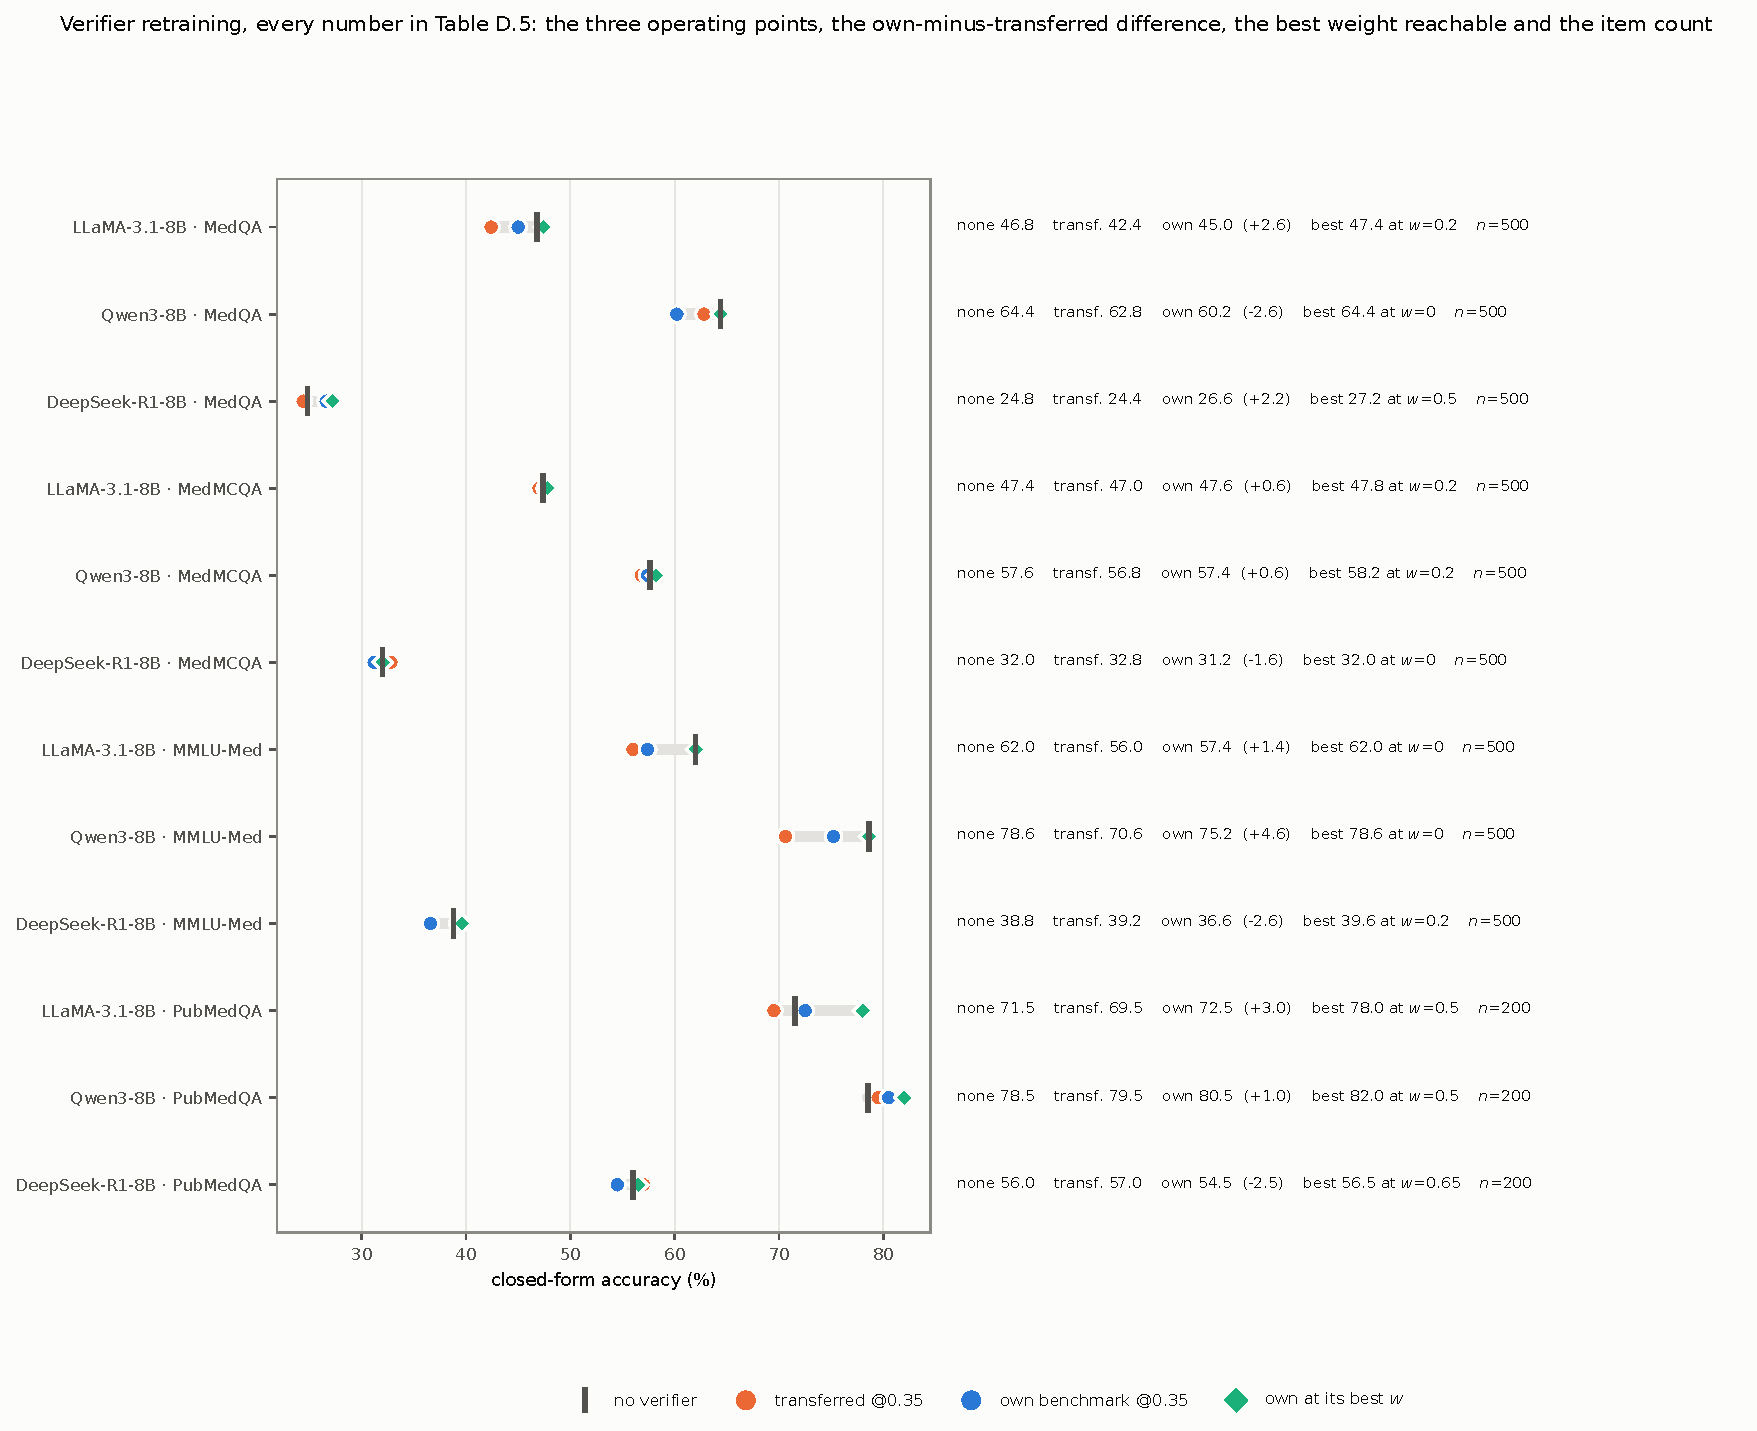
\includegraphics[width=\linewidth]{figures/tabD5_verifier_retrain_full.pdf}
\caption{Verifier retraining, every column of Table~\ref{tab:verifier-retrain}: the three operating points, the own-minus-transferred difference, the best weight reachable and the item count.}
\label{fig:tabD5-verifier-retrain-full}
\end{figure*}
